\subsection{View design (Magnus)}\label{sec:viewDesign}

We settled on the following four pages as part of the View (Fig \ref{fig:MVC_CD}): a login page, a create customer page, a customer page, and an admin page. For sample screenshots of these pages, see Appendix \ref{sec:appendixView}. Adhering to the MVC design pattern, these pages should be limited to presenting the current Model data. The user interacts with the application through a web browser. All communication with the Model should occur through the Control classes.

\begin{figure}[H]
\centering

\begin{subfigure}[b]{0.49\textwidth}
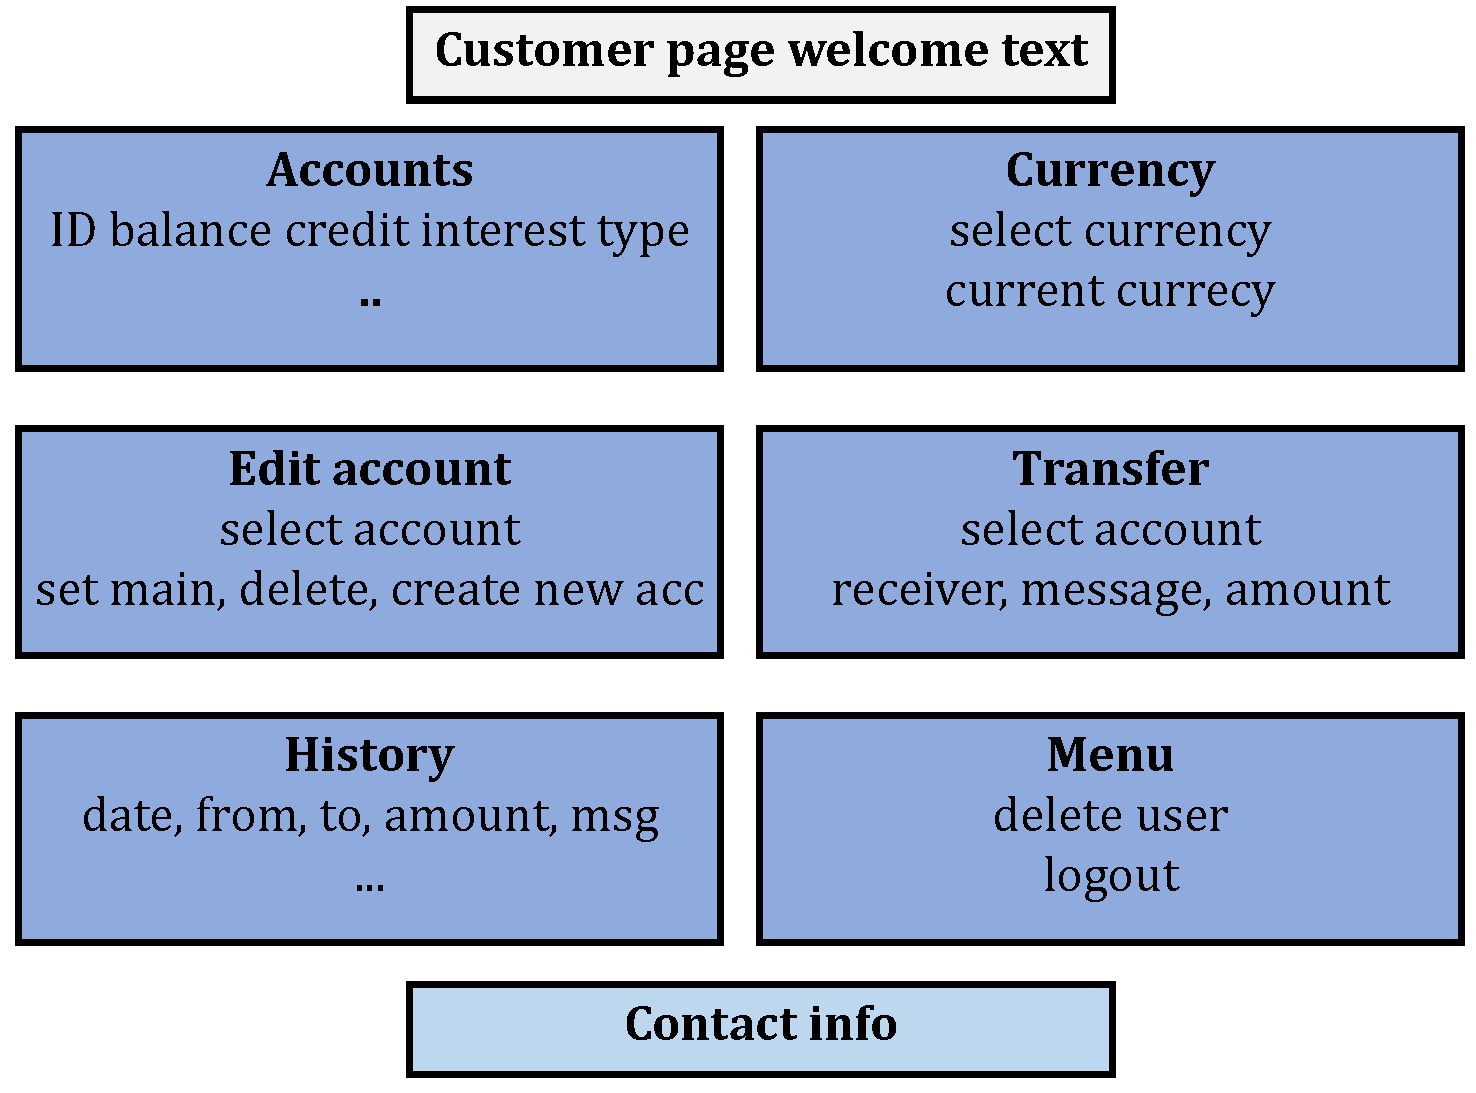
\includegraphics[width=\textwidth]{figures/customerPage.pdf}
\caption{Intended content in the customer page.}
\label{fig:customerPageDesign}
\end{subfigure}%
\hfill
\begin{subfigure}[b]{0.49\textwidth}
  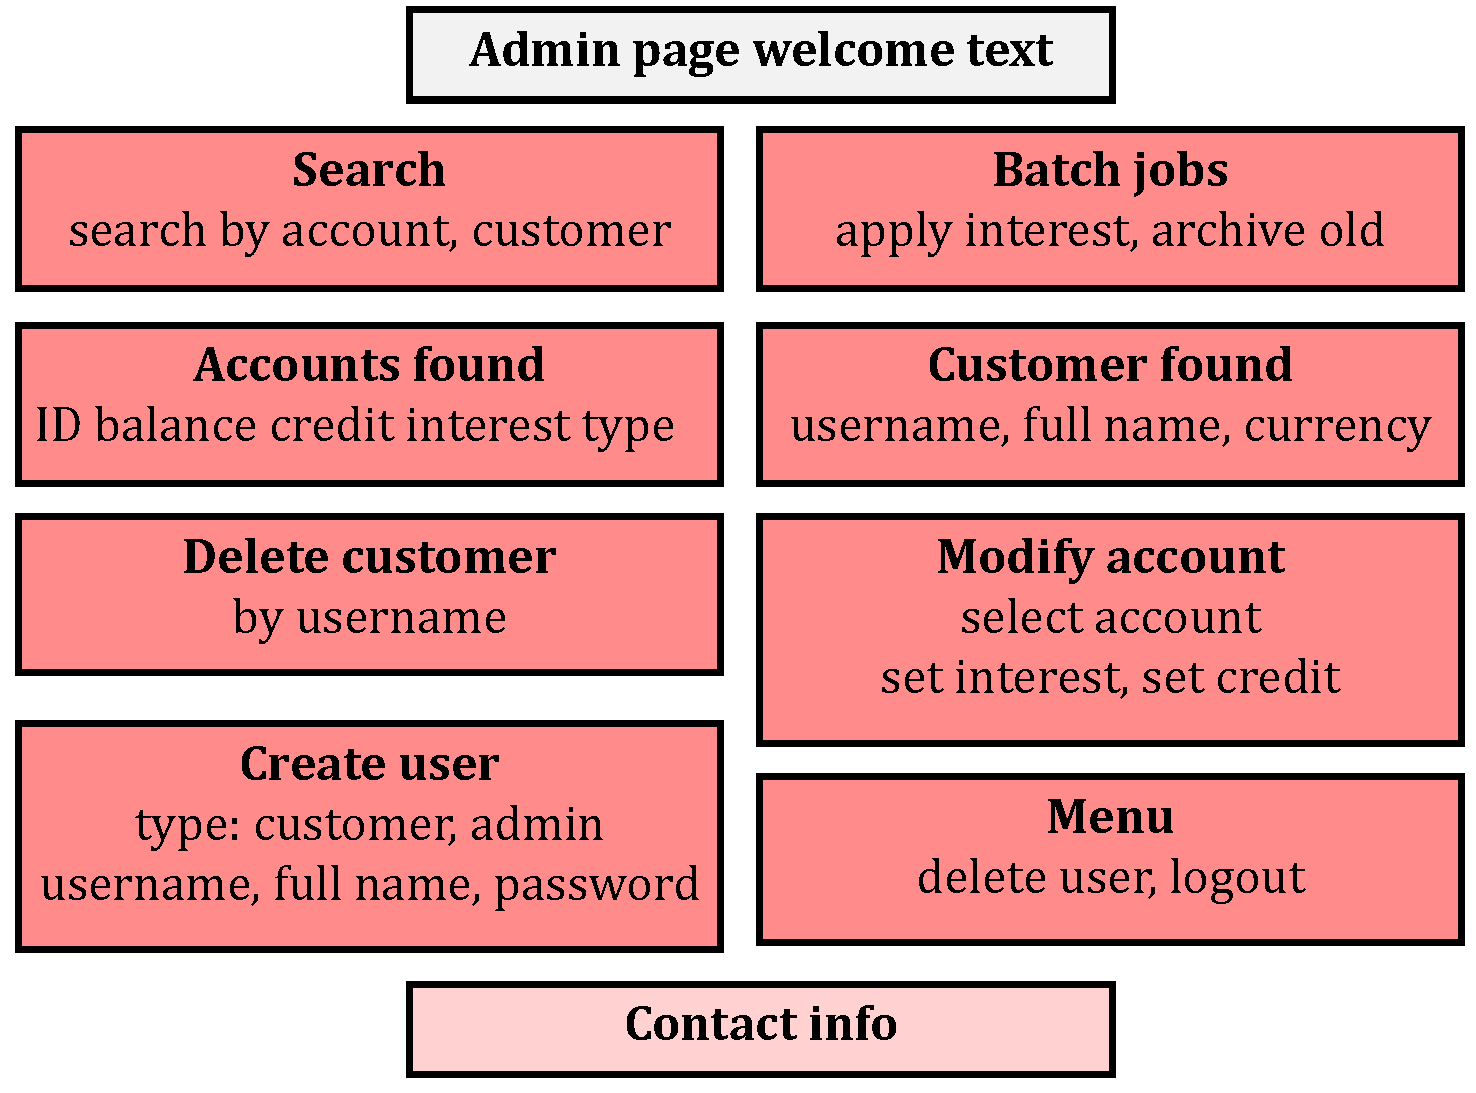
\includegraphics[width=\textwidth]{figures/adminPage.pdf}
\caption{Intended content in the admin page.}
\label{fig:adminPageDesign}
\end{subfigure}

\caption{View design: intended content in the two user pages.}
\end{figure}

\textbf{Dividing users:} Initially we considered just having a single user page. Upon login, the application should decide which buttons and actions should be accessible and shown. But as the project progressed, the divide between customer actions (e.g. transfer money) and admin actions (e.g. search) became prominent, so we divided the user page into two separate pages: customer page and admin page. The intended contents in the customer page and admin page are seen in Figs \ref{fig:customerPageDesign} and \ref{fig:adminPageDesign}. Account information should be shown as text, possibly through a \texttt{toString} method in an Account object.

\textbf{Errors:} When a user performs an illegal action, an error message should be shown to the user. This functionality can be integrated into Java exceptions, but should be displayed by View classes.